% !TeX root = RJwrapper.tex
\title{Variable Importance Plots---An Introduction to the \pkg{vip} Package}
\author{by Brandon M. Greenwell, Bradley C. Boehmke}

\maketitle

\abstract{%
In the era of ``big data'', it is becoming more of a challenge to not
only build state-of-the-art predictive models, but also gain an
understanding of what's really going on in the data. For example, it is
often of interest to know which, if any, of the predictors in a fitted
model are relatively influential on the predicted outcome. Some modern
algorithms---like random forests (RFs) and gradient boosted decision
trees (GBMs)---have a natural way of quantifying the importance or
relative influence of each feature. Other algorithms---like naive Bayes
classifiers and support vector machines---are not capable of doing so
and \dfn{model-agnostic approaches} are generally used to measure each
predictor's importance. Enter \pkg{vip}, an R package for constructing
variable importance scores/plots for many types of supervised learning
algorithms using model-specific and novel model-agnostic approaches.
We'll also discuss a novel way to display both feature importance and
feature effects together using \dfn{sparklines}, a very small line chart
conveying the general shape or variation in some feature that can be
directly embedded in text or tables.
}

\hypertarget{introduction}{%
\subsection{Introduction}\label{introduction}}

Too often machine learning (ML) models are summarized using a single
metric (e.g., cross-validated accuracy) and then put into production.
Although we often care about the predictions from these models, it is
becoming routine (and good practice) to also better understand the
predictions! Understanding how an ML model makes its predictions helps
build trust in the model and is the fundamental idea of the emerging
field of \dfn{interpretable machine learning} (IML).\footnote{Although
  ``interpretability'' is difficult to formally define in the context of
  ML, we follow \citet{doshivelez-2017-rigorous} and describe
  ``interpretable'' as the ``\ldots{}ability to explain or to present in
  understandable terms to a human.''} For an in-depth discussion on IML,
see \citet{molnar-2019-iml}. In this paper, we focus on
\dfn{global methods} for quantifying the importance\footnote{In this
  context ``importance'' can be defined in a number of different ways.
  In general, we can describe it as
  \dfn{the extent to which a feature has a "meaningful" impact on the predicted outcome}.
  A more formal definition and treatment can be found in
  \citet{laan-2006-statistical}.} of features in an ML model; that is,
methods that help us understand the global contribution each feature has
to a model's predictions. Computing variable importance (VI) and
communicating them through variable importance plots (VIPs) is a
fundamental component of IML and is the main topic of this paper.

While many of the procedures discussed in this paper apply to any model
that makes predictions, it should be noted that these methods heavily
depend on the accuracy and importance of the fitted model; hence,
unimportant features may appear relatively important (albeit not
predictive) in comparison to the other included features. For this
reason, we stress the usefulness of understanding the scale on which VI
scores are calculated and take that into account when assessing the
importance of each feature and communicating the results to others.
Also, we should point out that this work focuses mostly on
\emph{post-hoc interpretability} where a trained model is given and the
goal is to understand what features are driving the model's predictions.
Consequently, our work focuses on functional understanding of the model
in contrast to the lower-level mechanistic understanding
\citep{montavon-2018-methods}. That is, we seek to explain the
relationship between the model's prediction behavior and features
without explaining the full internal representation of the
model.\footnote{We refer the reader to \citet{poulin-2006-visual},
  \citet{caruana-2015-intelligible},
  \citet{bibal-2016-intterpretability}, and \citet{bau-2017-network},
  for discussions around model structure interpretation.}

VI scores and VIPs can be constructed for general ML models using a
number of available packages. The \CRANpkg{iml} package \citep{R-iml}
provides the \code{FeatureImp()} function which computes feature
importance for general prediction models using the permutation approach
(discussed later). It is written in \CRANpkg{R6} \citep{R-R6} and allows
the user to specify a generic loss function or select one from a
pre-defined list (e.g., \code{loss = "mse"} for mean squared error). It
also allows the user to specify whether importance is measured as the
difference or as the ratio of the original model error and the model
error after permutation. The user can also specify the number of
repetitions used when permuting each feature to help stabilize the
variability in the procedure. The \code{iml::FeatureImp()} function can
also be run in parallel using any parallel backend supported by the
\CRANpkg{foreach} package \citep{R-foreach}.

The \CRANpkg{ingredients} package \citep{R-ingredients} also provides
permutation-based VI scores through the \code{feature\_importance()}
function. (Note that this function recently replaced the now deprecated
\CRANpkg{DALEX} function \code{variable\_importance()} \citep{R-DALEX}.)
Similar to \code{iml::FeatureImp()}, this function allows the user to
specify a loss function and how the importance scores are computed
(e.g., using the difference or ratio). It also provides an option to
sample the training data before shuffling the data to compute importance
(the default is to use \code{n\_sample = 1000}), which can help speed up
computation.

The \CRANpkg{mmpf} package \citep{R-mmpf} also provides
permutation-based VI scores via the
\newline \code{mmpf::permutationImportance()} function. Similar to the
\pkg{iml} and \pkg{ingredients} implementation, this function is
flexible enough to be applied to any class of ML models in R.

The \CRANpkg{varImp} package \citep{R-varImp} extends the
permutation-based method for RFs in package \CRANpkg{party}
\citep{R-party} to arbitrary measures from the \CRANpkg{measures}
package \citep{R-measures}. Additionally, the functions in \pkg{varImp}
include the option of using the conditional approach described in
\citet{strobl-2019-conditional} which is more reliable in the presence
of correlated features. A number of other RF-specific VI packages exist
on CRAN, including, but not limited to, \CRANpkg{vita} \citep{R-vita},
\CRANpkg{rfVarImpOOB} \citep{R-rfVarImpOOB},
\CRANpkg{randomForestExplainer} \citep{R-randomForestExplainer}, and
\CRANpkg{tree.interpreter} \citep{R-tree.interpreter}.\footnote{These
  packages were discovered using \CRANpkg{pkgsearch}'s \code{ps()}
  function \citep{R-pkgsearch} with the key phrases ``variable
  importance'' and ``feature importance''.}.

The \CRANpkg{caret} package \citep{R-caret} includes a general
\code{varImp()} function for computing model-specific and
\dfn{filter-based} VI scores. Filter-based approaches, which are
described in \citet{applied-kuhn-2013}, do not make use of the fitted
model to measure VI. They also do not take into account the other
predictors in the model. For regression problems, a popular filter-based
approach to measuring the VI of a numeric predictor \(x\) is to first
fit a flexible nonparametric model between \(x\) and the target \(Y\);
for example, the locally-weighted polynomial regression (LOWESS) method
developed by \citet{robust-cleveland-1979}. From this fit, a
pseudo-\(R^2\) measure can be obtained from the resulting residuals and
used as a measure of VI. For categorical predictors, a different method
based on standard statistical tests (e.g., \(t\)-tests and ANOVAs) can
be employed; see \citet{applied-kuhn-2013} for details. For
classification problems, an area under the ROC curve (AUC) statistic can
be used to quantify predictor importance. The AUC statistic is computed
by using the predictor \(x\) as input to the ROC curve. If \(x\) can
reasonably separate the classes of \(Y\), that is a clear indicator that
\(x\) is an important predictor (in terms of class separation) and this
is captured in the corresponding AUC statistic. For problems with more
than two classes, extensions of the ROC curve or a one-vs-all approach
can be used.

If you use the \CRANpkg{mlr} interface for fitting ML models
\citep{R-mlr}, then you can use the \code{getFeatureImportance()}
function to extract model-specific VI scores from various tree-based
models (e.g., RFs and GBMs). Unlike \pkg{caret}, the model needs to be
fit via the \pkg{mlr} interface; for instance, you cannot use
\code{getFeatureImportance()} on a \CRANpkg{ranger} \citep{R-ranger}
model unless it was fit using \pkg{mlr}.

While the \pkg{iml} and \pkg{DALEX} packages provide model-agnostic
approaches to computing VI, \pkg{caret}, and to some extent, \pkg{mlr},
provide model-specific approaches (e.g., using the absolute value of the
\(t\)-statistic for linear models) as well as less accurate filter-based
approaches. Furthermore, each package has a completely different
interface (e.g., \pkg{iml} is written in R6). The \CRANpkg{vip} package
\citep{R-vip} strives to provide a consistent interface to both
model-specific and model-agnostic approaches to feature importance that
is simple to use. The three most important functions exported by
\pkg{vip} are described below:

\begin{itemize}

  \item \code{vi()} computes VI scores using model-specific or model-agnostic approaches (the results are always returned as a tibble \citep{R-tibble});

  \item \code{vip()} constructs VIPs using model-specific or model-agnostic approaches with \CRANpkg{ggplot2}-style graphics \citep{R-ggplot2};

  \item \code{add\_sparklines()} adds a novel sparkline representation of feature effects (e.g., \dfn{partial dependence plots}) to any VI table produced by \code{vi()}.

\end{itemize}

There's also a function called \code{vint()} (for variable interactions)
but it is experimental and will not be discussed here; the interested
reader is pointed to \citet{greenwell-simple-2018}. Note that
\code{vi()} is actually a wrapper around four workhorse functions,
\code{vi\_model()}, \code{vi\_firm()}, \code{vi\_permute()}, and
\code{vi\_shap()}, that compute various types of VI scores. The first
computes model-specific VI scores, while the latter three produce
model-agnostic ones. The workhorse function that actually gets called is
controlled by the \code{method} argument in \code{vi()}; the default is
\code{method = "model"} which corresponds to model-specific VI (see
\code{?vip::vi} for details and links to further documentation).

\hypertarget{constructing-vips-in-r}{%
\subsection{Constructing VIPs in R}\label{constructing-vips-in-r}}

We'll illustrate major concepts using the Friedman 1 benchmark problem
described in \citet{multivariate-friedman-1991} and
\citet{bagging-breiman-1996}:

\begin{equation}
  Y_i = 10 \sin\left(\pi X_{1i} X_{2i}\right) + 20 \left(X_{3i} - 0.5\right) ^ 2 + 10 X_{4i} + 5 X_{5i} + \epsilon_i, \quad i = 1, 2, \dots, n,
\label{eqn:friedman1}
\end{equation}

where \(\epsilon_i \stackrel{iid}{\sim} N\left(0, \sigma^2\right)\).
Data from this model can be generated using the
\code{vip::gen\_friedman()}. By default, the features consist of 10
independent variables uniformly distributed on the interval
\(\left[0,1\right]\); however, only 5 out of these 10 are actually used
in the true model. The code chunk below simulates 500 observations from
the model in Equation \eqref{eqn:friedman1} with \(\sigma = 1\); see
\code{?vip::gen\_friedman} for details.

\begin{Schunk}
\begin{Sinput}
trn <- vip::gen_friedman(500, sigma = 1, seed = 101)  # simulate training data
tibble::as_tibble(trn)  # inspect output
\end{Sinput}
\begin{Soutput}
#> # A tibble: 500 x 11
#>        y     x1    x2    x3    x4     x5      x6    x7    x8    x9   x10
#>    <dbl>  <dbl> <dbl> <dbl> <dbl>  <dbl>   <dbl> <dbl> <dbl> <dbl> <dbl>
#>  1 14.9  0.372  0.406 0.102 0.322 0.693  0.758   0.518 0.530 0.878 0.763
#>  2 15.3  0.0438 0.602 0.602 0.999 0.776  0.533   0.509 0.487 0.118 0.176
#>  3 15.1  0.710  0.362 0.254 0.548 0.0180 0.765   0.715 0.844 0.334 0.118
#>  4 10.7  0.658  0.291 0.542 0.327 0.230  0.301   0.177 0.346 0.474 0.283
#>  5 17.6  0.250  0.794 0.383 0.947 0.462  0.00487 0.270 0.114 0.489 0.311
#>  6 18.3  0.300  0.701 0.992 0.386 0.666  0.198   0.924 0.775 0.736 0.974
#>  7 14.6  0.585  0.365 0.283 0.488 0.845  0.466   0.715 0.202 0.905 0.640
#>  8 17.0  0.333  0.552 0.858 0.509 0.697  0.388   0.260 0.355 0.517 0.165
#>  9  8.54 0.622  0.118 0.490 0.390 0.468  0.360   0.572 0.891 0.682 0.717
#> 10 15.0  0.546  0.150 0.476 0.706 0.829  0.373   0.192 0.873 0.456 0.694
#> # ... with 490 more rows
\end{Soutput}
\end{Schunk}

From Equation \eqref{eqn:friedman1}, it should be clear that features
\(X_1\)--\(X_5\) are the most important! (The others don't influence
\(Y\) at all.) Also, based on the form of the model, we'd expect \(X_4\)
to be the most important feature, probably followed by \(X_1\) and
\(X_2\) (both comparably important), with \(X_5\) probably being less
important. The influence of \(X_3\) is harder to determine due to its
quadratic nature, but it seems likely that this nonlinearity will
suppress the variable's influence over its observed range (i.e., 0--1).

\section{Model-specific VI}

Some machine learning algorithms have their own way of quantifying the
importance of each feature, which we refer to as
\dfn{model-specific VI}. We describe some of these in the subsections
that follow. One particular issue with model-specific VI scores is that
they are not necessarily comparable across different types of models.
For example, directly comparing the impurity-based VI scores from
tree-based models to the the absolute value of the \(t\)-statistic in
linear models.

\subsection{Decision trees and tree ensembles}

Decision trees probably offer the most natural model-specific approach
to quantifying the importance of each feature. In a binary decision
tree, at each node \(t\), a single predictor is used to partition the
data into two homogeneous groups. The chosen predictor is the one that
maximizes some measure of improvement \(i^t\). The relative importance
of predictor \(X\) is the sum of the squared improvements over all
internal nodes of the tree for which \(X\) was chosen as the
partitioning variable; see \citet{classification-breiman-1984} for
details. This idea also extends to ensembles of decision trees, such as
RFs and GBMs. In ensembles, the improvement score for each predictor is
averaged across all the trees in the ensemble. Fortunately, due to the
stabilizing effect of averaging, the improvement-based VI metric is
often more reliable in large ensembles; see
\citet[p. 368]{hastie-elements-2009}.

RFs offer an additional method for computing VI scores. The idea is to
use the leftover \dfn{out-of-bag} (OOB) data to construct validation-set
errors for each tree. Then, each predictor is randomly shuffled in the
OOB data and the error is computed again. The idea is that if variable
\(X\) is important, then the validation error will go up when \(X\) is
perturbed in the OOB data. The difference in the two errors is recorded
for the OOB data then averaged across all trees in the forest. Note that
both methods for constructing VI scores can be unreliable in certain
situations; for example, when the predictor variables vary in their
scale of measurement or their number of categories \citep{party2007a},
or when the predictors are highly correlated
\citep{strobl-2019-conditional}. The \pkg{varImp} package discussed
earlier provides methods to address these concerns for random forests in
package \pkg{party}, with similar functionality also built into the
\CRANpkg{partykit} package \citep{R-partykit}. The \pkg{vip} package
also supports the conditional importance described in
\citep{strobl-2019-conditional} for both \pkg{party}- and
\pkg{partykit}-based RFs; see \texttt{?vip::vi\_model} for details.
Later on, we'll discuss a more general permutation method that can be
applied to any supervised learning model.

To illustrate, we fit a CART-like regression tree, RF, and GBM to the
simulated training data. (\strong{Note:} there are a number of different
packages available for fitting these types of models, we just picked
popular implementations for illustration.)

\begin{Schunk}
\begin{Sinput}
# Load required packages
library(rpart)          # for fitting CART-like decision trees
library(randomForest)   # for fitting RFs
library(xgboost)        # for fitting GBMs

# Fit a single regression tree
tree <- rpart(y ~ ., data = trn)

# Fit an RF
set.seed(101)  # for reproducibility
rfo <- randomForest(y ~ ., data = trn, importance = TRUE)

# Fit a GBM
set.seed(102)  # for reproducibility
bst <- xgboost(
  data = data.matrix(subset(trn, select = -y)),
  label = trn$y,
  objective = "reg:squarederror",
  nrounds = 100,
  max_depth = 5,
  eta = 0.3,
  verbose = 0  # suppress printing
)
\end{Sinput}
\end{Schunk}

Each of the above packages include the ability to compute VI scores for
all the features in the model; however, the implementation is rather
package-specific, as shown in the code chunk below. The results are
displayed in Figure \ref{fig:vi-plots} (the code to reproduce these
plots has been omitted but can be made available upon request).

\begin{Schunk}
\begin{Sinput}
# Extract VI scores from each model
vi_tree <- tree$variable.importance
vi_rfo <- rfo$variable.importance  # or use `randomForest::importance(rfo)`
vi_bst <- xgb.importance(model = bst)
\end{Sinput}
\end{Schunk}

\begin{Schunk}
\begin{figure}[!htb]

{\centering 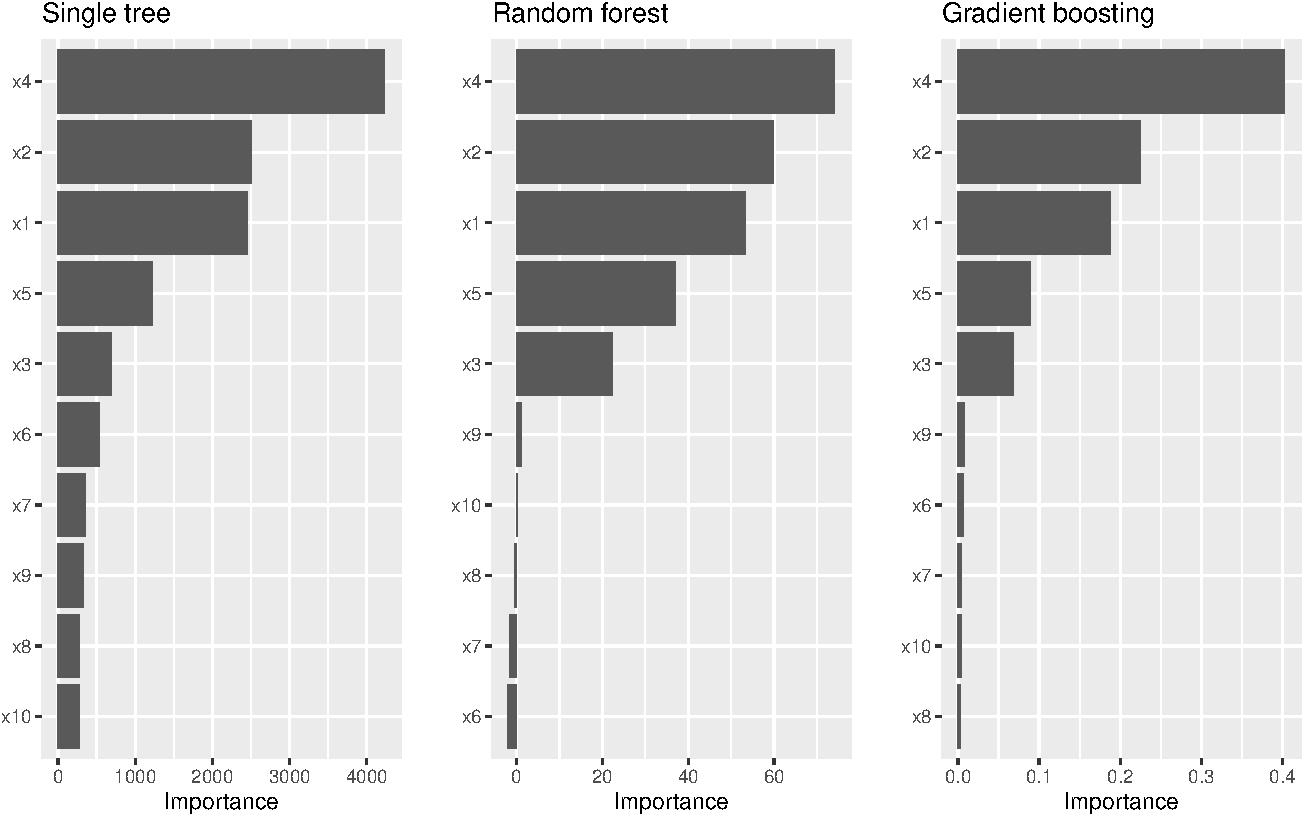
\includegraphics[width=1\linewidth]{greenwell-boehmke_files/figure-latex/vi-plots-1}

}

\caption[Model-specific VIPs for the three different tree-based models fit to the simulated Friedman data]{Model-specific VIPs for the three different tree-based models fit to the simulated Friedman data.}\label{fig:vi-plots}
\end{figure}
\end{Schunk}

As we would expect, all three methods rank the variables
\code{x1}--\code{x5} as more important than the others. While this is
good news, it is unfortunate that we have to remember the different
functions and ways of extracting and plotting VI scores from various
model fitting functions. This is one place where \pkg{vip} can
help\ldots{}one function to rule them all! Once \pkg{vip} is loaded, we
can use \code{vi()} to extract a tibble of VI scores.

\begin{Schunk}
\begin{Sinput}
# Load required packages
library(vip)

# Compute model-specific VI scores
vi(tree)  # CART-like decision tree
\end{Sinput}
\begin{Soutput}
#> # A tibble: 10 x 2
#>    Variable Importance
#>    <chr>         <dbl>
#>  1 x4            4234.
#>  2 x2            2513.
#>  3 x1            2461.
#>  4 x5            1230.
#>  5 x3             688.
#>  6 x6             533.
#>  7 x7             357.
#>  8 x9             331.
#>  9 x8             276.
#> 10 x10            275.
\end{Soutput}
\begin{Sinput}
vi(rfo)   # RF
\end{Sinput}
\begin{Soutput}
#> # A tibble: 10 x 2
#>    Variable Importance
#>    <chr>         <dbl>
#>  1 x4           74.2
#>  2 x2           59.9
#>  3 x1           53.3
#>  4 x5           37.1
#>  5 x3           22.5
#>  6 x9            1.05
#>  7 x10           0.254
#>  8 x8           -0.408
#>  9 x7           -1.56
#> 10 x6           -2.00
\end{Soutput}
\begin{Sinput}
vi(bst)   # GBM
\end{Sinput}
\begin{Soutput}
#> # A tibble: 10 x 2
#>    Variable Importance
#>    <chr>         <dbl>
#>  1 x4          0.403
#>  2 x2          0.225
#>  3 x1          0.189
#>  4 x5          0.0894
#>  5 x3          0.0682
#>  6 x9          0.00802
#>  7 x6          0.00746
#>  8 x7          0.00400
#>  9 x10         0.00377
#> 10 x8          0.00262
\end{Soutput}
\end{Schunk}

Notice how the \code{vi()} function always returns a
tibble\footnote{Technically, it's a tibble with an additional \code{"vi"} class.}
with two columns: \code{Variable} and \code{Importance} (the exceptions
are coefficient-based models which also include a \code{Sign} column
giving the sign of the corresponding coefficient, and permutation
importance involving multiple Monte Carlo simulations, but more on that
later). Also, by default, \code{vi()} always orders the VI scores from
highest to lowest; this, among other options, can be controlled by the
user (see \code{?vip::vi} for details). Plotting VI scores with
\code{vip()} is just as straightforward. For example, the following code
can be used to reproduce Figure \ref{fig:vi-plots}.

\begin{Schunk}
\begin{Sinput}
p1 <- vip(tree) + ggtitle("Single tree")
p2 <- vip(rfo) + ggtitle("Random forest")
p3 <- vip(bst) + ggtitle("Gradient boosting")

# Display plots in a grid (Figure 1)
grid.arrange(p1, p2, p3, nrow = 1)
\end{Sinput}
\end{Schunk}

Notice how the \code{vip()} function always returns a \code{"ggplot"}
object (by default, this will be a bar plot). For large models with many
features, a Cleveland dot plot is more effective (in fact, a number of
useful plotting options can be fiddled with). Below we call \code{vip()}
and change a few useful options (the resulting plot is displayed in
Figure \ref{fig:dot-plot}). Note that we can also call \code{vip()}
directly on a \code{"vi"} object if it's already been constructed.

\begin{Schunk}
\begin{Sinput}
# Construct VIP (Figure 2)
library(ggplot2)  # for theme_light() function
vip(bst, num_features = 5, geom = "point", horizontal = FALSE,
    aesthetics = list(color = "red", shape = 17, size = 5)) +
  theme_light()
\end{Sinput}
\begin{figure}[!htb]

{\centering 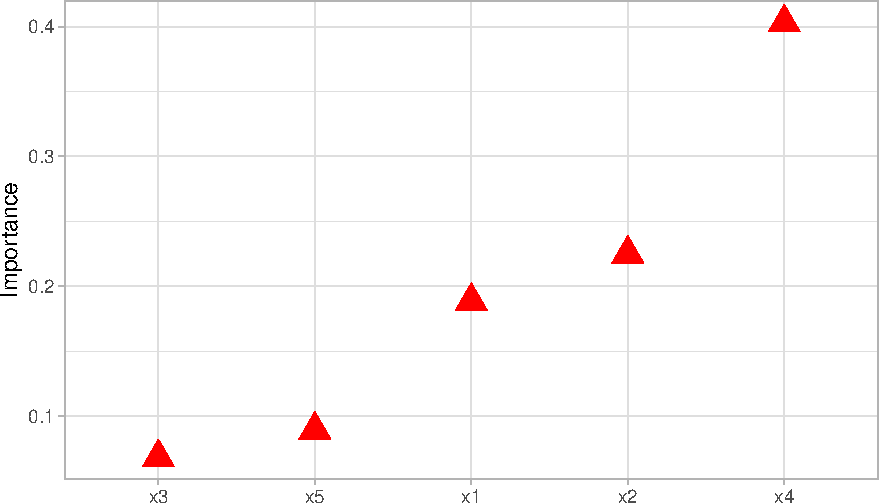
\includegraphics[width=0.7\linewidth]{greenwell-boehmke_files/figure-latex/dot-plot-1}

}

\caption[Illustrating various plotting options]{Illustrating various plotting options.}\label{fig:dot-plot}
\end{figure}
\end{Schunk}

\hypertarget{linear-models}{%
\subsection{Linear models}\label{linear-models}}

In multiple linear regression, or linear models (LMs), the absolute
value of the \(t\)-statistic (or some other scaled variant of the
estimated coefficients) is commonly used as a measure of VI.\footnote{Since
  this approach is biased towards large-scale features it is important
  to properly standardize the predictors (before fitting the model) or
  the estimated coefficients.} The same idea also extends to generalized
linear models (GLMs). In the code chunk below, we fit an LM to the
simulated Friedman data (\texttt{trn}) allowing for all main effects and
two-way interactions, then use the \code{step()} function to perform
backward elimination. The resulting VIP is displayed in Figure
\ref{fig:vip-step}.

\begin{Schunk}
\begin{Sinput}
# Fit a LM
linmod <- lm(y ~ .^2, data = trn)
backward <- step(linmod, direction = "backward", trace = 0)

# Extract VI scores
(vi_backward <- vi(backward))
\end{Sinput}
\begin{Soutput}
#> # A tibble: 21 x 3
#>    Variable Importance Sign
#>    <chr>         <dbl> <chr>
#>  1 x4            14.2  POS
#>  2 x2             7.31 POS
#>  3 x1             5.63 POS
#>  4 x5             5.21 POS
#>  5 x3:x5          2.46 POS
#>  6 x1:x10         2.41 NEG
#>  7 x2:x6          2.41 NEG
#>  8 x1:x5          2.37 NEG
#>  9 x10            2.21 POS
#> 10 x3:x4          2.01 NEG
#> # ... with 11 more rows
\end{Soutput}
\begin{Sinput}
# Plot VI scores; by default, `vip()` displays the top ten features
vip(vi_backward, num_features = length(coef(backward)),  # Figure 3
    geom = "point", horizontal = FALSE, mapping = aes(color = Sign)) +
  theme(axis.text.x = element_text(angle = 45, hjust = 1))
\end{Sinput}
\begin{figure}[!htb]

{\centering 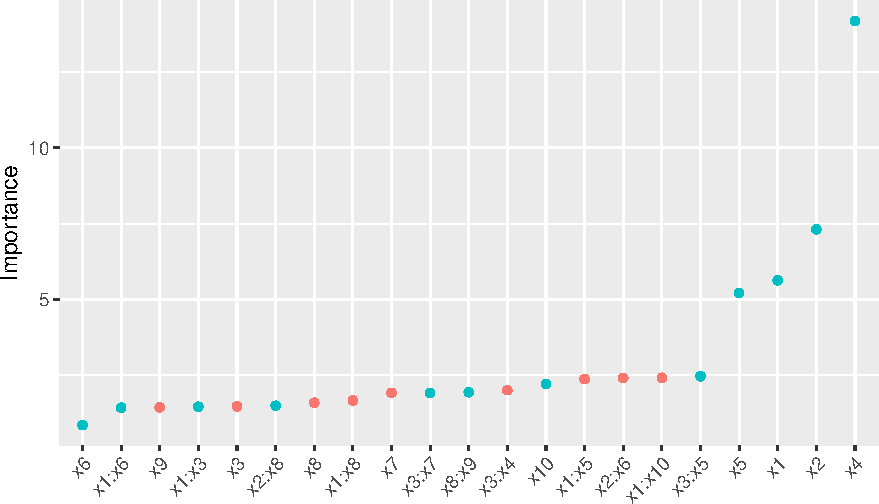
\includegraphics[width=0.7\linewidth]{greenwell-boehmke_files/figure-latex/vip-step-1}

}

\caption[Example VIP from a linear model fit to the simulated Friedman data]{Example VIP from a linear model fit to the simulated Friedman data. The points are colored according to the sign of the associated coefficient.}\label{fig:vip-step}
\end{figure}
\end{Schunk}

A major limitation of this approach is that a VI score is assigned to
each term in the model, rather than to each individual feature! We can
solve this problem using one of the model-agnostic approaches discussed
later.

Multivariate adaptive regression splines (MARS), which were introduced
in \citet{multivariate-friedman-1991}, is an automatic regression
technique and can be seen as a generalization of LMs and GLMs. In the
MARS algorithm, the contribution (or VI score) for each predictor is
determined using a generalized cross-validation (GCV) statistic (though,
other statistics can also be used; see \code{?vip::vi\_model} for
details). An example using the \CRANpkg{earth} package
\citep{R-earth-fixed} is given below (the results are plotted in Figure
\ref{fig:vip-earth}):

\begin{Schunk}
\begin{Sinput}
# Load required packages
library(earth)

# Fit a MARS model
mars <- earth(y ~ ., data = trn, degree = 2, pmethod = "exhaustive")

# Extract VI scores
vi(mars, type = "gcv")
\end{Sinput}
\begin{Soutput}
#> # A tibble: 10 x 2
#>    Variable Importance
#>    <chr>         <dbl>
#>  1 x4            100
#>  2 x1             83.2
#>  3 x2             83.2
#>  4 x5             59.3
#>  5 x3             43.5
#>  6 x6              0
#>  7 x7              0
#>  8 x8              0
#>  9 x9              0
#> 10 x10             0
\end{Soutput}
\begin{Sinput}
# Plot VI scores (Figure 4)
vip(mars)
\end{Sinput}
\begin{figure}[!htb]

{\centering 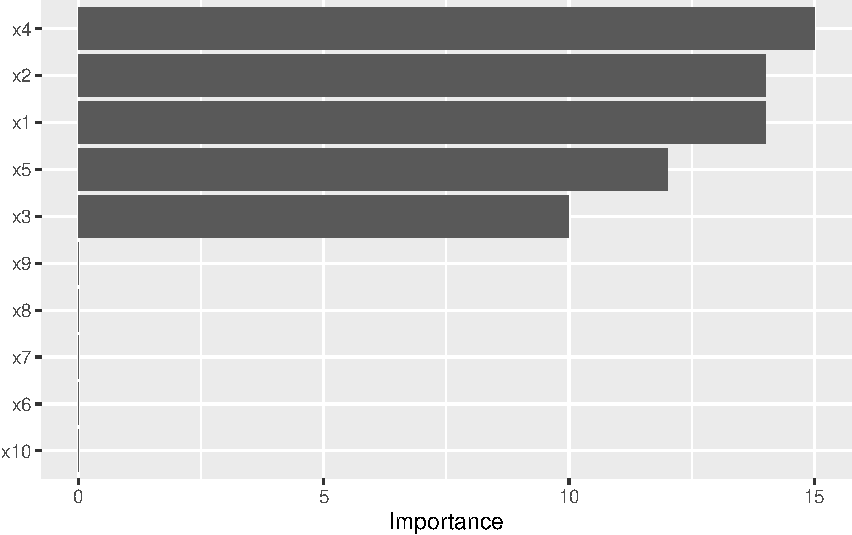
\includegraphics[width=0.7\linewidth]{greenwell-boehmke_files/figure-latex/vip-earth-1}

}

\caption[Example VIP from a MARS model fit to the simulated Friedman data]{Example VIP from a MARS model fit to the simulated Friedman data.}\label{fig:vip-earth}
\end{figure}
\end{Schunk}

To access VI scores directly in \pkg{earth}, you can use the
\code{earth::evimp()} function.

\hypertarget{neural-networks}{%
\subsection{Neural networks}\label{neural-networks}}

For neural networks (NNs), two popular methods for constructing VI
scores are the Garson algorithm \citep{interpreting-garson-1991}, later
modified by \citet{back-goh-1995}, and the Olden algorithm
\citep{accurate-olden-2004}. For both algorithms, the basis of these VI
scores is the network's connection weights. The Garson algorithm
determines VI by identifying all weighted connections between the nodes
of interest. Olden's algorithm, on the other hand, uses the products of
the raw connection weights between each input and output neuron and sums
these products across all hidden neurons. This has been shown to
outperform the Garson method in various simulations. For DNNs, a similar
method due to \citet{data-gedeon-1997} considers the weights connecting
the input features to the first two hidden layers (for simplicity and
speed); but this method can be slow for large networks. We illustrate
these two methods below using \code{vip()} with the \CRANpkg{nnet}
package \citep{R-nnet} (see the results in Figure \ref{fig:vip-nnet}).

\begin{Schunk}
\begin{Sinput}
# Load required packages
library(nnet)

# Fit a neural network
set.seed(0803)  # for reproducibility
nn <- nnet(y ~ ., data = trn, size = 7, decay = 0.1,
           linout = TRUE, trace = FALSE)

# Construct VIPs
p1 <- vip(nn, type = "garson")
p2 <- vip(nn, type = "olden")

# Display plots in a grid (Figure 5)
grid.arrange(p1, p2, nrow = 1)
\end{Sinput}
\begin{figure}[!htb]

{\centering 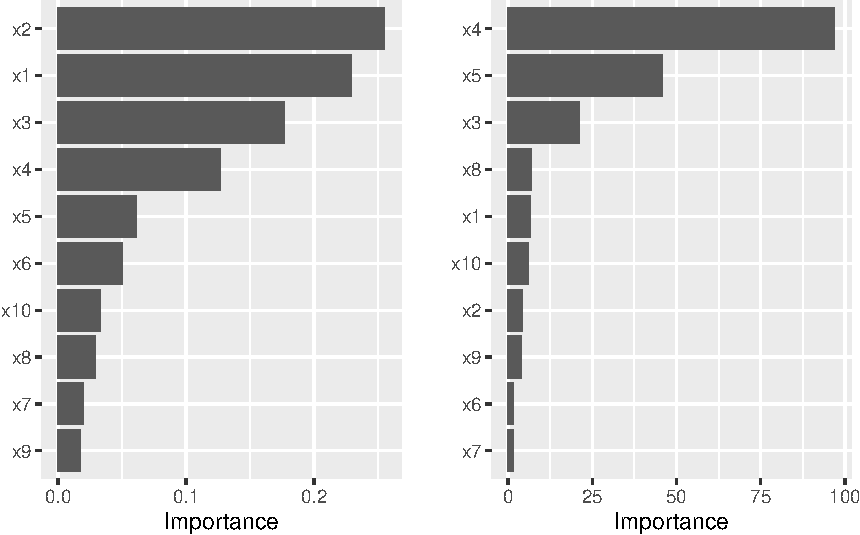
\includegraphics[width=0.7\linewidth]{greenwell-boehmke_files/figure-latex/vip-nnet-1}

}

\caption[Example VIPs from a single-hidden-layer NN fit to the simulated Friedman data]{Example VIPs from a single-hidden-layer NN fit to the simulated Friedman data.}\label{fig:vip-nnet}
\end{figure}
\end{Schunk}

\section{Model-agnostic VI}

Model-agnostic interpretability separates interpretation from the model.
Compared to model-specific approaches, model-agnostic VI methods are
more flexible and can be applied to any supervised learning algorithm.
In this section, we discuss model-agnostic methods for quantifying
global feature importance using three different approaches: 1) a simple
variance-based approach, 2) permutation-based feature importance, and 3)
Shapley-based feature importance.

\subsection{Variance-based methods}

Our first model-agnostic method is based on a simple \emph{feature
importance ranking measure} (FIRM); for details, see
\citet{greenwell-simple-2018}, \citet{zien-2009-feature}, and
\citet{scholbeck-2019-sampling}. The specific approach used here is
based on quantifying the ``flatness'' of the effects of each
feature.\footnote{A similar approach is taken in the \CRANpkg{vivo}
  package \citep{R-vivo}.} Feature effects can be assessed using
\emph{partial dependence plots} (PDPs) \citep{friedman-2001-greedy} or
\emph{individual conditional expectation} (ICE) curves
\citep{goldstein-peeking-2015}. PDPs and ICE curves help visualize the
effect of low cardinality subsets of the feature space on the estimated
prediction surface (e.g., main effects and two/three-way interaction
effects.). They are also model-agnostic and can be constructed in the
same way for any supervised learning algorithm. Below, we fit a
\dfn{projection pursuit regression} (PPR) model (see
\texttt{?stats::ppr} for details and references) and construct PDPs for
each feature using the \CRANpkg{pdp} package \citet{pdp2017}. The
results are displayed in Figure \ref{fig:pdp-ppr}. Notice how the PDPs
for the uninformative features are relatively flat compared to the PDPs
for features \code{x1}--\code{x5}!

\begin{Schunk}
\begin{figure}[!htb]

{\centering 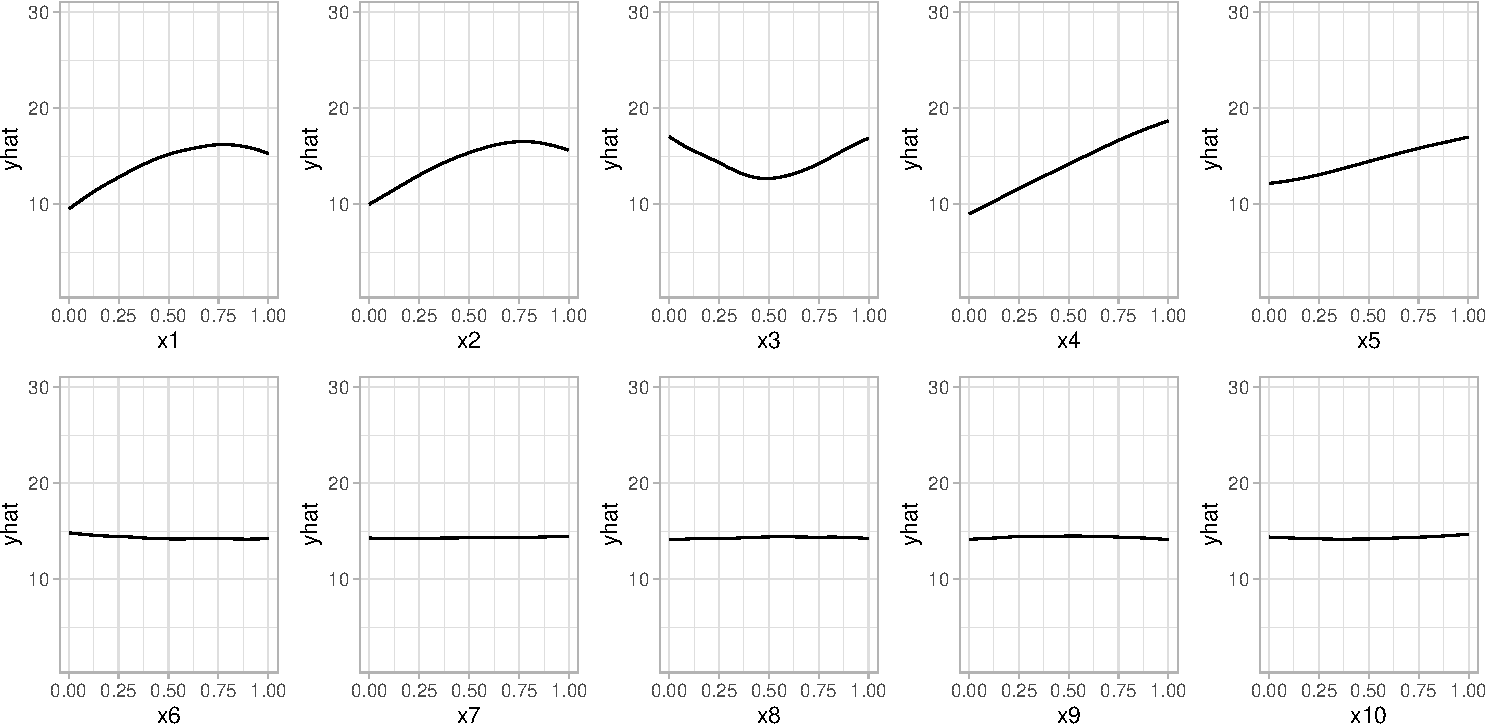
\includegraphics[width=1\linewidth]{greenwell-boehmke_files/figure-latex/pdp-ppr-1}

}

\caption[PDPs of main effects in the PPR model fit to the simulated Friedman data]{PDPs of main effects in the PPR model fit to the simulated Friedman data.}\label{fig:pdp-ppr}
\end{figure}
\end{Schunk}

Next, we compute PDP-based VI scores for the fitted PPR and NN models.
The PDP method constructs VI scores that quantify the relative
``flatness'' of each PDP (by default, this is defined by computing the
standard deviation of the \(y\)-axis values for each PDP). To use the
PDP method, specify \code{method = "firm"} in the call to \code{vi()} or
\code{vip()} (or just use \code{vi\_firm()} directly):

\begin{Schunk}
\begin{Sinput}
# Fit a PPR model (nterms was chosen using the caret package with 5 repeats of
# 5-fold cross-validation)
pp <- ppr(y ~ ., data = trn, nterms = 11)

# Construct VIPs
p1 <- vip(pp, method = "firm") + ggtitle("PPR")
p2 <- vip(nn, method = "firm") + ggtitle("NN")

# Display plots in a grid (Figure 7)
grid.arrange(p1, p2, ncol = 2)
\end{Sinput}
\begin{figure}[!htb]

{\centering 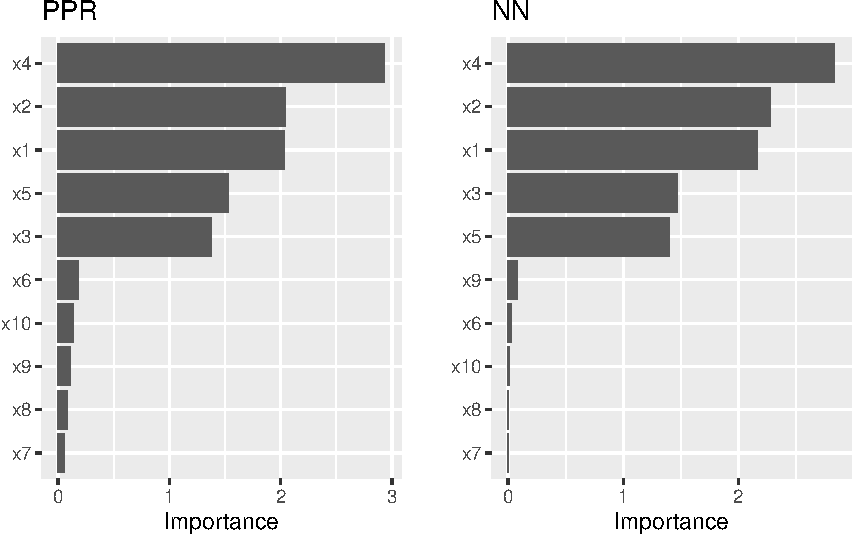
\includegraphics[width=0.7\linewidth]{greenwell-boehmke_files/figure-latex/pdp-ppr-nn-1}

}

\caption[PDP-based feature importance for the PPR and NN models fit to the simulated Friedman data]{PDP-based feature importance for the PPR and NN models fit to the simulated Friedman data.}\label{fig:pdp-ppr-nn}
\end{figure}
\end{Schunk}

In Figure \ref{fig:pdp-ppr-nn} we display the PDP-based feature
importance for the previously obtained PPR and NN models. These VI
scores essentially capture the variability in the partial dependence
values for each main effect.

The ICE curve method is similar to the PDP method, except that we
measure the ``flatness'' of each individual ICE curve and then aggregate
the results (e.g., by averaging). If there are no (substantial)
interaction effects, using ICE curves will produce results similar to
using PDPs (which are just averaged ICE curves). However, if strong
interaction effects are present, they can obfuscate the main effects and
render the PDP-based approach less useful (since the PDPs for important
features can be relatively flat when certain interactions are present;
see \citet{goldstein-peeking-2015} for details). In fact, it is probably
safest to always use ICE curves when employing the FIRM method.

Below, we display the ICE curves for each feature in the fitted PPR
model using the same \(y\)-axis scale; see Figure \ref{fig:ice-ppr}.
Again, there is a clear difference between the ICE curves for features
\code{x1}--\code{x5} and \code{x6}--\code{x10}; the later being
relatively flat by comparison. Also, notice how the ICE curves within
each feature are relatively parallel (if the ICE curves within each
feature were perfectly parallel, the standard deviation for each curve
would be the same and the results will be identical to the PDP method).
In this example, the interaction term between \code{x1} and \code{x2}
does not obfuscate the PDPs for the main effects and the results are not
much different.

\begin{Schunk}
\begin{figure}[!htb]

{\centering 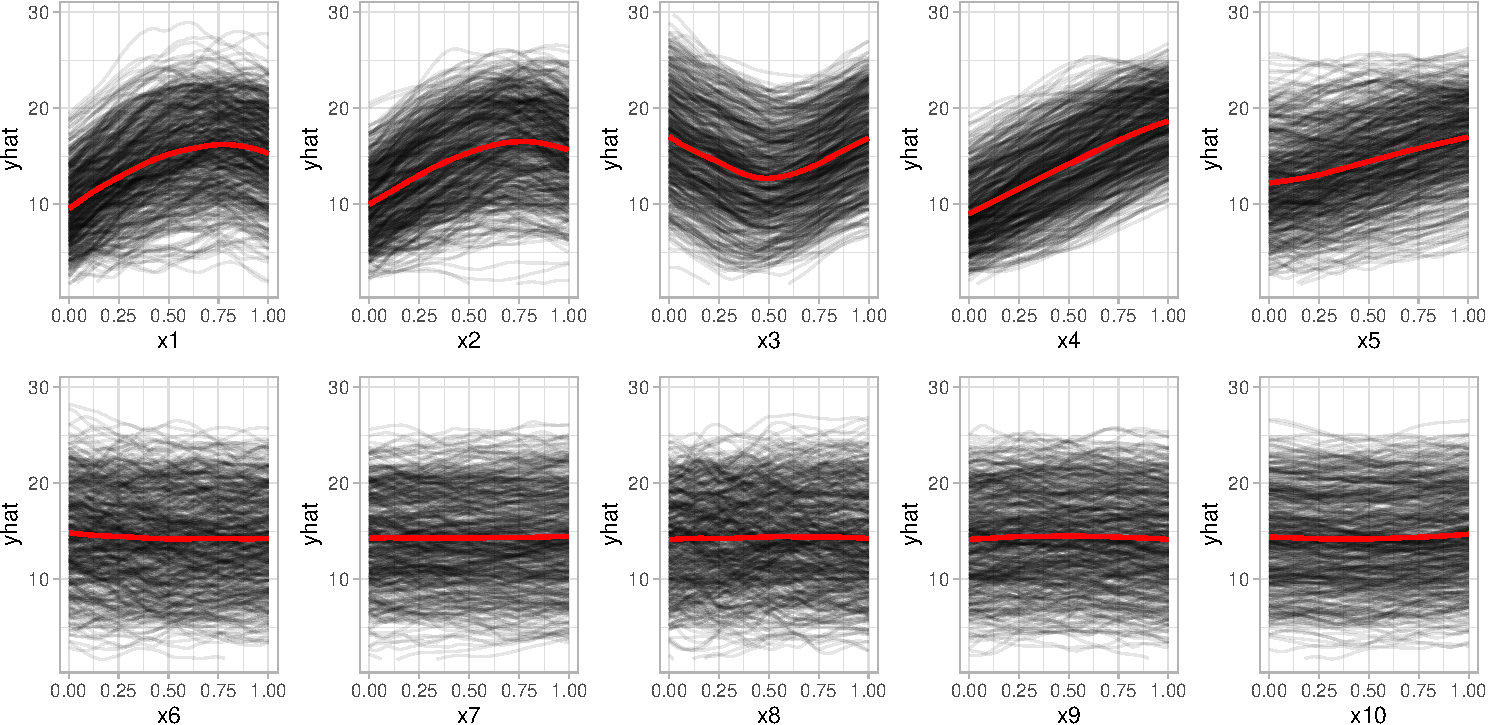
\includegraphics[width=1\linewidth]{greenwell-boehmke_files/figure-latex/ice-ppr-1}

}

\caption[ICE curves for each feature in the PPR model fit to the simulated Friedman data]{ICE curves for each feature in the PPR model fit to the simulated Friedman data. The red curve represents the PDP (i.e., the averaged ICE curves).}\label{fig:ice-ppr}
\end{figure}
\end{Schunk}

Obtaining the ICE-based feature importance scores is also
straightforward, just specify \code{ice = TRUE} when using the FIRM
approach. This is illustrated in the code chunk below and the results,
which are displayed in Figure \ref{fig:vip-ice-ppr-nn}, are similar to
those obtained using the PDP method.

\begin{Schunk}
\begin{Sinput}
# Construct VIPs
p1 <- vip(pp, method = "firm", ice = TRUE) + ggtitle("PPR")
p2 <- vip(nn, method = "firm", ice = TRUE) + ggtitle("NN")

# Display plots in a grid (Figure 9)
grid.arrange(p1, p2, ncol = 2)
\end{Sinput}
\begin{figure}[!htb]

{\centering 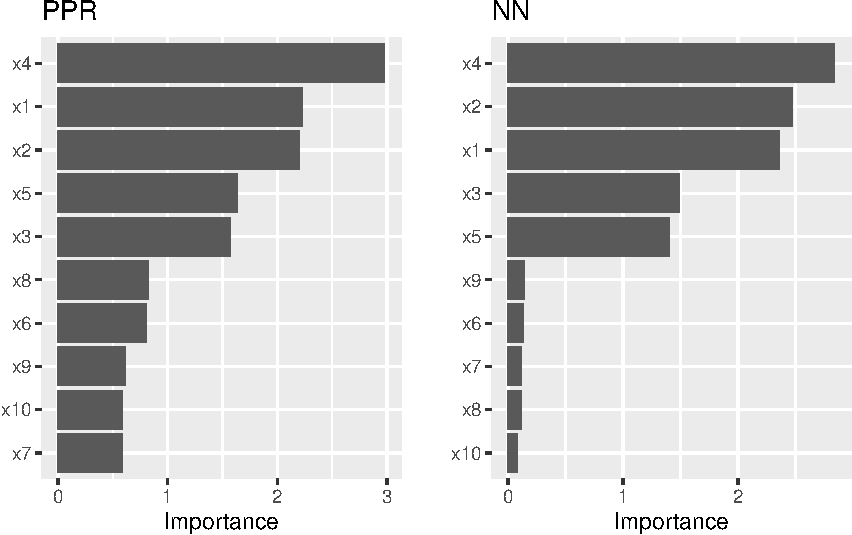
\includegraphics[width=0.7\linewidth]{greenwell-boehmke_files/figure-latex/vip-ice-ppr-nn-1}

}

\caption[ICE-based feature importance for the PPR and NN models fit to the simulated Friedman data]{ICE-based feature importance for the PPR and NN models fit to the simulated Friedman data.}\label{fig:vip-ice-ppr-nn}
\end{figure}
\end{Schunk}

When using \code{method = "firm"}, the feature effect values are stored
in an attribute called \code{"effects"}. This is a convenience so that
the feature effect plots (e.g., PDPs and ICE curves) can easily be
reconstructed and compared with the VI scores, as demonstrated in the
example below (see Figure \ref{fig:pdp-from-attr}):

\begin{Schunk}
\begin{Sinput}
# Construct PDP-based VI scores
(vis <- vi(pp, method = "firm"))
\end{Sinput}
\begin{Soutput}
#> # A tibble: 10 x 2
#>    Variable Importance
#>    <chr>         <dbl>
#>  1 x4           2.93
#>  2 x2           2.05
#>  3 x1           2.04
#>  4 x5           1.53
#>  5 x3           1.38
#>  6 x6           0.183
#>  7 x10          0.139
#>  8 x9           0.113
#>  9 x8           0.0899
#> 10 x7           0.0558
\end{Soutput}
\begin{Sinput}
# Reconstruct PDPs for all 10 features (Figure 10)
par(mfrow = c(2, 5))
for (name in paste0("x", 1:10)) {
  plot(attr(vis, which = "effects")[[name]], type = "l", ylim = c(9, 19), las = 1)
}
\end{Sinput}
\begin{figure}[!htb]

{\centering 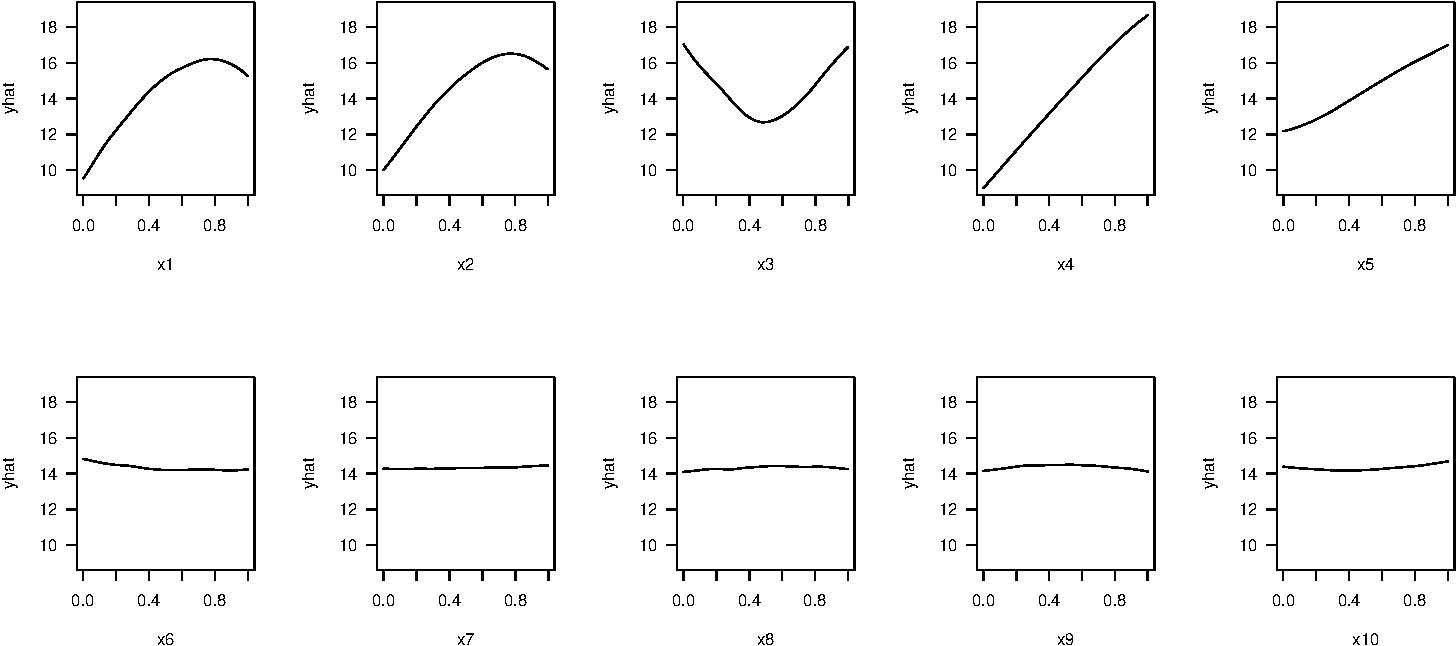
\includegraphics[width=1\linewidth]{greenwell-boehmke_files/figure-latex/pdp-from-attr-1}

}

\caption[PDPs for all ten features reconstructed from the \code{pdp} attribute of the \code{vis} object]{PDPs for all ten features reconstructed from the \code{pdp} attribute of the \code{vis} object.}\label{fig:pdp-from-attr}
\end{figure}
\end{Schunk}

\subsection{Permutation method}

The permutation method exists in various forms and was made popular in
\citet{random-breiman-2001} for RFs, before being generalized and
extended in \citet{fisher-model-2018}. The permutation approach used in
\pkg{vip} is quite simple and is outlined in Algorithm \ref{alg:permute}
below. The idea is that if we randomly permute the values of an
important feature in the training data, the training performance would
degrade (since permuting the values of a feature effectively destroys
any relationship between that feature and the target variable). This of
course assumes that the model has been properly tuned (e.g., using
cross-validation) and is not over fitting. The permutation approach uses
the difference between some baseline performance measure (e.g., training
\(R^2\), AUC, or RMSE) and the same performance measure obtained after
permuting the values of a particular feature in the training data
(\strong{Note:} the model is NOT refit to the training data after
randomly permuting the values of a feature). It is also important to
note that this method may not be appropriate when you have, for example,
highly correlated features (since permuting one feature at a time may
lead to unlikely data instances).

Let \(X_1, X_2, \dots, X_j\) be the features of interest and let
\(\mathcal{M}_{orig}\) be the baseline performance metric for the
trained model; for brevity, we'll assume smaller is better (e.g.,
classification error or RMSE). The permutation-based importance scores
can be computed as follows:

\begin{algorithm}
\begin{enumerate}
  \item For $i = 1, 2, \dots, j$:
  \begin{enumerate}
    \item Permute the values of feature $X_i$ in the training data.
    \item Recompute the performance metric on the permuted data $\mathcal{M}_{perm}$.
    \item Record the difference from baseline using $imp\left(X_i\right) = \mathcal{M}_{perm} - \mathcal{M}_{orig}$.
  \end{enumerate}
  \item Return the VI scores $imp\left(X_1\right), imp\left(X_2\right), \dots, imp\left(X_j\right)$.
\end{enumerate}
\caption{A simple algorithm for constructing permutation-based VI scores. \label{alg:permute}}
\end{algorithm}

Algorithm \ref{alg:permute} can be improved or modified in a number of
ways. For instance, the process can be repeated several times and the
results averaged together. This helps to provide more stable VI scores,
and also the opportunity to measure their variability. Rather than
taking the difference in step (c), \citet[sec. 5.5.4]{molnar-2019-iml}
argues that using the ratio \(\mathcal{M}_{perm} / \mathcal{M}_{orig}\)
makes the importance scores more comparable across different problems.
It's also possible to assign importance scores to groups of features
(e.g., by permuting more than one feature at a time); this would be
useful if features can be categorized into mutually exclusive groups,
for instance, categorical features that have been \dfn{one-hot-encoded}.

To use the permutation approach in \pkg{vip}, specify
\code{method = "permute"} in the call to \code{vi()} or \code{vip()} (or
you can use \texttt{vi\_permute()} directly). Note that using
\code{method = "permute"} requires specifying a few additional arguments
(e.g., the training data, target name or vector of target values, a
prediction function, etc.); see \code{?vi\_permute} for details.

An example is given below for the previously fitted PPR and NN models.
Here we use \(R^2\) (\code{metric = "rsquared"}) as the evaluation
metric. The results, which are displayed in Figure
\ref{fig:vip-permute-ppr-nn}, agree with those obtained using the PDP-
and ICE-based methods.

\begin{Schunk}
\begin{Sinput}
# Plot VI scores
set.seed(2021)  # for reproducibility
p1 <- vip(pp, method = "permute", target = "y", metric = "rsquared",
          pred_wrapper = predict) + ggtitle("PPR")
p2 <- vip(nn, method = "permute", target = "y", metric = "rsquared",
          pred_wrapper = predict) + ggtitle("NN")

# Display plots in a grid (Figure 11)
grid.arrange(p1, p2, ncol = 2)
\end{Sinput}
\begin{figure}[!htb]

{\centering 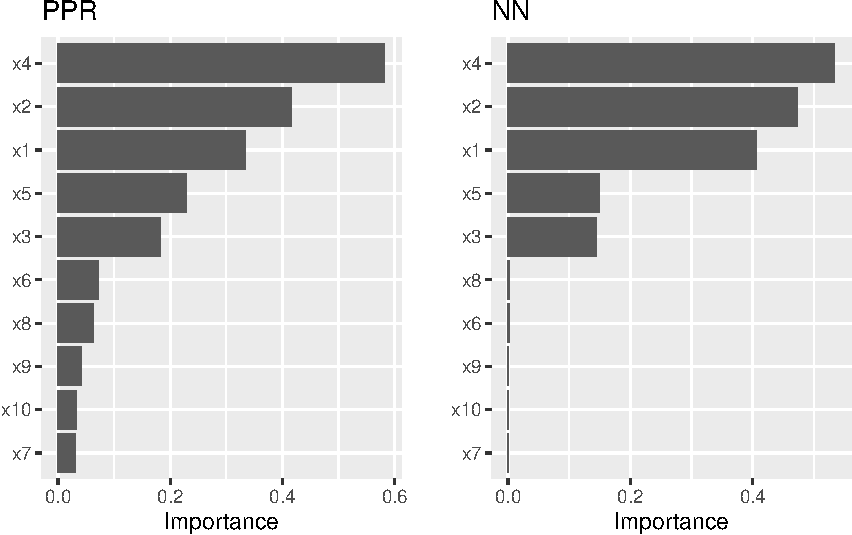
\includegraphics[width=0.7\linewidth]{greenwell-boehmke_files/figure-latex/vip-permute-ppr-nn-1}

}

\caption[Permutation-based feature importance for the PPR and NN models fit to the simulated Friedman data]{Permutation-based feature importance for the PPR and NN models fit to the simulated Friedman data.}\label{fig:vip-permute-ppr-nn}
\end{figure}
\end{Schunk}

The permutation approach introduces randomness into the procedure and
therefore should be run more than once if computationally feasible. The
upside to performing multiple runs of Algorithm \ref{alg:permute} is
that it allows us to compute standard errors (among other metrics) for
the estimated VI scores, as illustrated in the example below; here we
specify \code{nsim = 10} to request that each feature be permuted 10
times and the results averaged together. (Additionally, if
\code{nsim > 1}, you can set \code{geom = "boxplot"} in the call to
\code{vip()} to construct boxplots of the raw permutation-based VI
scores. This is useful if you want to visualize the variability in each
of the VI estimates; see Figure \ref{fig:vip-boxplots} for an example.)

\begin{Schunk}
\begin{Sinput}
# Use 10 Monte Carlo reps
set.seed(403)  # for reproducibility
vis <- vi(pp, method = "permute", target = "y", metric = "rsquared",
          pred_wrapper = predict, nsim = 15)
vip(vis, geom = "boxplot")  # Figure 12
\end{Sinput}
\begin{figure}[!htb]

{\centering 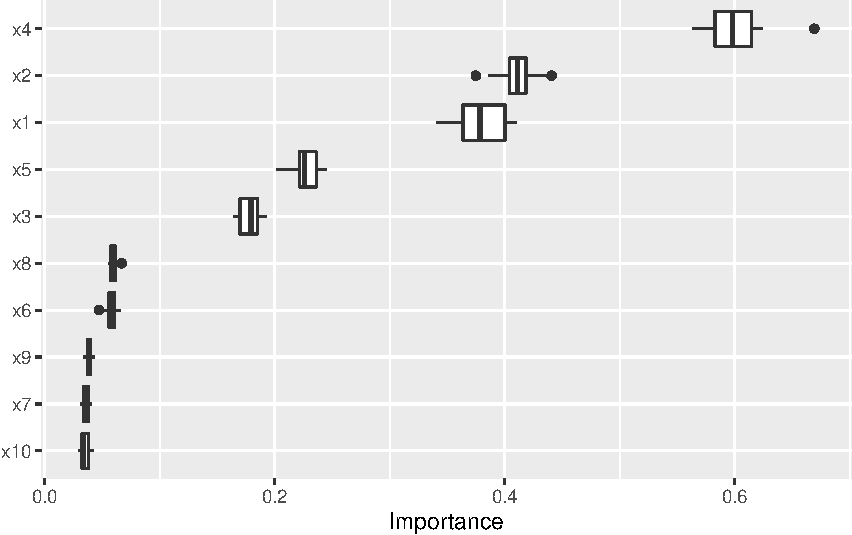
\includegraphics[width=0.7\linewidth]{greenwell-boehmke_files/figure-latex/vip-boxplots-1}

}

\caption[Boxplots of VI scores using the permutation method with 15 Monte Carlo repetitions]{Boxplots of VI scores using the permutation method with 15 Monte Carlo repetitions.}\label{fig:vip-boxplots}
\end{figure}
\end{Schunk}

All available performance metrics for regression and classification can
be listed using the \code{list\_metrics()} function, for example:

\begin{Schunk}
\begin{Sinput}
list_metrics()
\end{Sinput}
\begin{Soutput}
#>      Metric                       Description                             Task
#> 1  accuracy           Classification accuracy Binary/multiclass classification
#> 2     error           Misclassification error Binary/multiclass classification
#> 3       auc            Area under (ROC) curve            Binary classification
#> 4   logloss                          Log loss            Binary classification
#> 5      mauc Multiclass area under (ROC) curve        Multiclass classification
#> 6       mae               Mean absolute error                       Regression
#> 7       mse                Mean squared error                       Regression
#> 8        r2                         R squared                       Regression
#> 9  rsquared                         R squared                       Regression
#> 10     rmse           Root mean squared error                       Regression
#> 11      sse             Sum of squared errors                       Regression
\end{Soutput}
\end{Schunk}

We can also use a custom metric (i.e., loss function). Suppose for
example you want to measure importance using the
\dfn{mean absolute error} (MAE):

\begin{equation}
  MAE = \frac{1}{n}\sum_{i = 1}^n\left|Y_i - \widehat{f}\left(\boldsymbol{X}_i\right)\right|,
\end{equation}

where \(\widehat{f}\left(\boldsymbol{X}_i\right)\) is the predicted
value of \(Y_i\). A simple function implementing this metric is given
below (note that, according to the documentation in \code{?vi\_permute},
user-supplied metric functions require two arguments: \code{actual} and
\code{predicted}).

\begin{Schunk}
\begin{Sinput}
mae <- function(actual, predicted) {
  mean(abs(actual - predicted))
}
\end{Sinput}
\end{Schunk}

To use this for computing permutation-based VI scores just pass it via
the \code{metric} argument (be warned, however, that the metric used for
computing permutation importance should be the same as the metric used
to train and tune the model). Also, since this is a custom metric, we
need to specify whether a smaller value indicates better performance by
setting \code{smaller\_is\_better = TRUE}. The results, which are
displayed in Figure \ref{fig:vip-nn-mae}, are similar to those in Figure
\ref{fig:vip-permute-ppr-nn}, albeit a different scale.

\begin{Schunk}
\begin{Sinput}
# Construct VIP (Figure 13)
set.seed(2321)  # for reproducibility
pfun <- function(object, newdata)  predict(object, newdata = newdata)
vip(nn, method = "permute", target = "y", metric = mae,
    smaller_is_better = TRUE, pred_wrapper = pfun) +
  ggtitle("Custom loss function: MAE")
\end{Sinput}
\begin{figure}[!htb]

{\centering 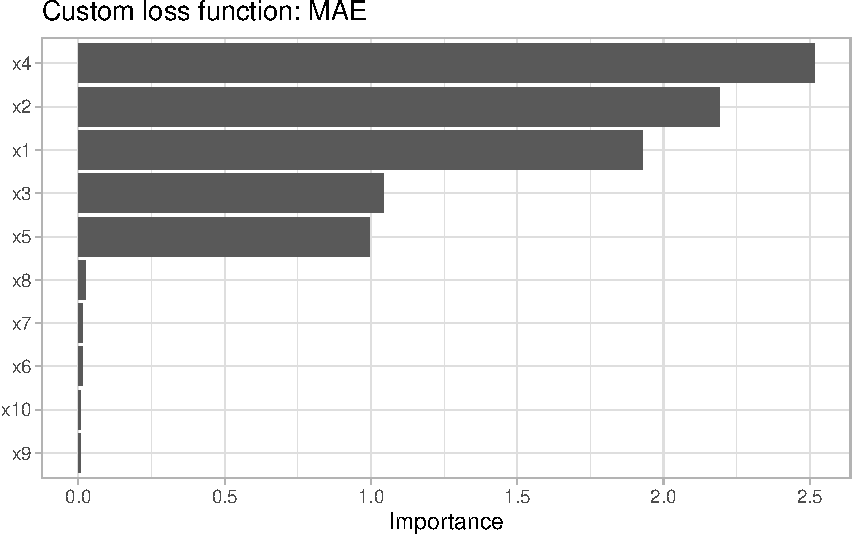
\includegraphics[width=0.7\linewidth]{greenwell-boehmke_files/figure-latex/vip-nn-mae-1}

}

\caption[Permutation-based VI scores for the NN model fit to the simulated Friedman data]{Permutation-based VI scores for the NN model fit to the simulated Friedman data. In this example, permutation importance is based on the MAE metric.}\label{fig:vip-nn-mae}
\end{figure}
\end{Schunk}

Although permutation importance is most naturally computed on the
training data, it may also be useful to do the shuffling and measure
performance on new data! This is discussed in depth in
\citet[sec. 5.2]{molnar-2019-iml}. For users interested in computing
permutation importance using new data, just supply it to the
\code{train} argument in the call to \code{vi()}, \code{vip()}, or
\code{vi\_permute()}. For instance, suppose we wanted to only use a
fraction of the original training data to carry out the computations. In
this case, we could simply pass the sampled data to the \code{train}
argument as follows:

\begin{Schunk}
\begin{Sinput}
# Construct VIP (Figure 14)
set.seed(2327)  # for reproducibility
vip(nn, method = "permute", pred_wrapper = pfun, target = "y", metric = "rmse",
    train = trn[sample(nrow(trn), size = 400), ]) +  # sample 400 observations
  ggtitle("Using a random subset of training data")
\end{Sinput}
\begin{figure}[!htb]

{\centering 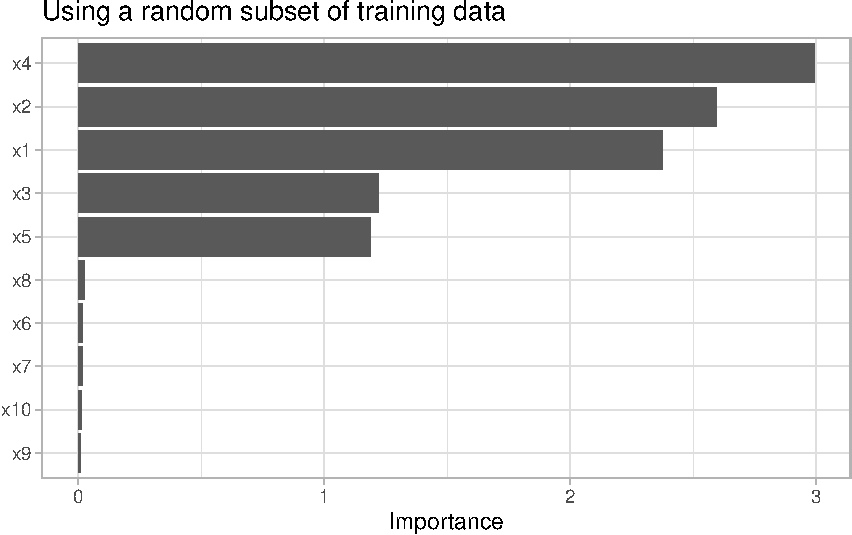
\includegraphics[width=0.7\linewidth]{greenwell-boehmke_files/figure-latex/vip-permute-nn-sample-1}

}

\caption[Permutation-based feature importance for the NN model fit to the simulated Friedman data]{Permutation-based feature importance for the NN model fit to the simulated Friedman data. In this example, permutation importance is based on a random sample of 400 training observations.}\label{fig:vip-permute-nn-sample}
\end{figure}
\end{Schunk}

When using the permutation method with \code{nsim > 1}, the default is
to keep all the permutation scores as an attribute called
\code{"raw\_scores"}; you can turn this behavior off by setting
\code{keep = FALSE} in the call to \code{vi\_permute()}, \code{vi()}, or
\code{vip()}. If \code{keep = TRUE} and \code{nsim > 1}, you can request
all permutation scores to be plotted by setting
\code{all\_permutation = TRUE} in the call to \code{vip()}, as
demonstrated in the code chunk below (see Figure
\ref{fig:vip-nn-mae-all}). This also let's you visually inspect the
variability in the permutation scores within each feature.

\begin{Schunk}
\begin{Sinput}
# Construct VIP (Figure 15)
set.seed(8264)  # for reproducibility
vip(nn, method = "permute", pred_wrapper = pfun, target = "y", metric = "mae",
    nsim = 10, geom = "point", all_permutations = TRUE, jitter = TRUE) +
  ggtitle("Plotting all permutation scores")
\end{Sinput}
\begin{figure}[!htb]

{\centering 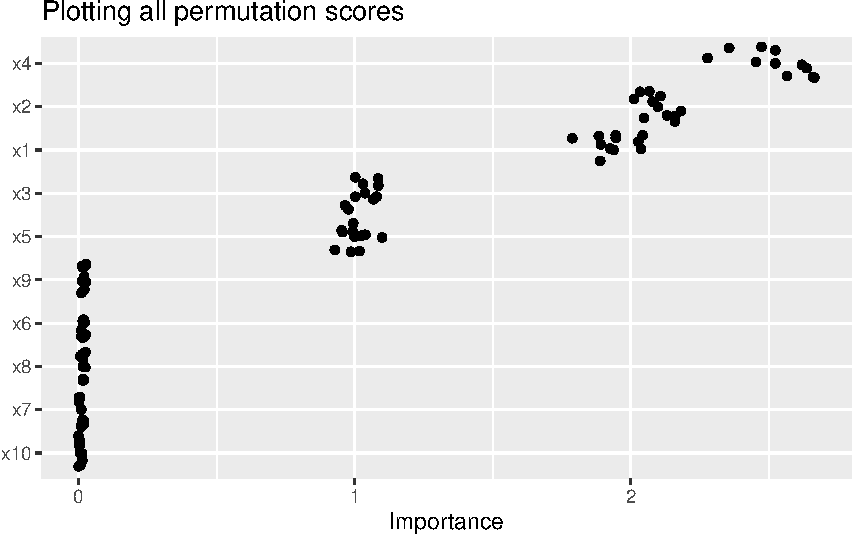
\includegraphics[width=0.7\linewidth]{greenwell-boehmke_files/figure-latex/vip-nn-mae-all-1}

}

\caption[Permutation-based feature importance for the NN model fit to the simulated Friedman data]{Permutation-based feature importance for the NN model fit to the simulated Friedman data. In this example, all the permutation importance scores (points) are displayed for each feature along with their average (bars).}\label{fig:vip-nn-mae-all}
\end{figure}
\end{Schunk}

\subsubsection{Benchmarks}

In this section, we compare the performance of four implementations of
permutation-based VI scores: \code{iml::FeatureImp()} (version 0.9.0),
\code{ingredients::feature\_importance()} (version 0.5.0),
\newline \code{mmpf::permutationImportance} (version 0.0.5), and
\code{vip::vi()} (version 0.2.1).

We simulated 10,000 training observations from the Friedman 1 benchmark
problem and trained a random forest using the \pkg{ranger} package. For
each implementation, we computed permutation-based VI scores 100 times
using the \CRANpkg{microbenchmark} package \citep{R-microbenchmark}. For
this benchmark we did not use any of the parallel processing capability
available in the \pkg{iml} and \pkg{vip} implementations. The results
from \pkg{microbenchmark} are displayed in Figure \ref{fig:benchmark}
and summarized in the output below. In this case, the \pkg{vip} package
(version 0.2.1) was the fastest, followed closely by \pkg{ingredients}
and \pkg{mmpf}. It should be noted, however, that the implementations in
\pkg{vip} and \pkg{iml} can be parallelized. To the best of our
knowledge, this is not the case for \pkg{ingredients} or \pkg{mmpf}
(although it would not be difficult to write a simple parallel wrapper
for either). The code used to generate these benchmarks can be found at
\url{http://bit.ly/2TogXrq}.

\begin{Schunk}
\begin{figure}[!htb]

{\centering 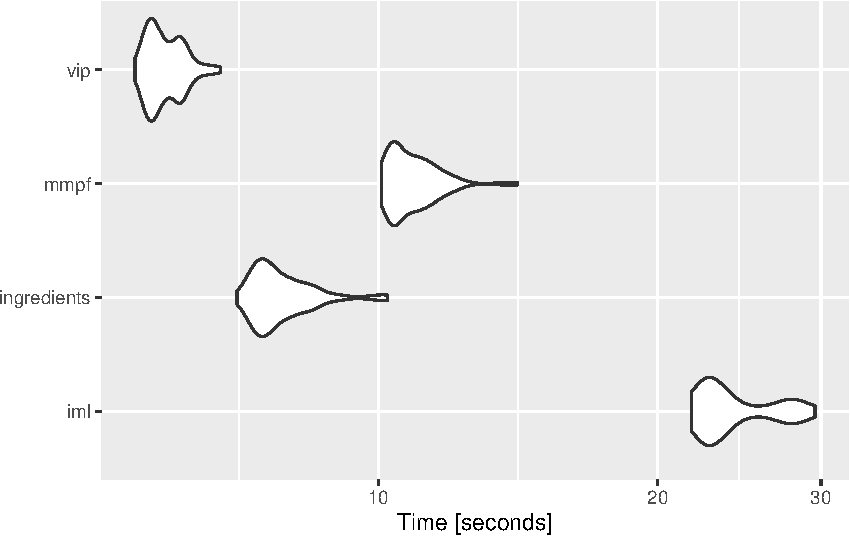
\includegraphics[width=0.7\linewidth]{greenwell-boehmke_files/figure-latex/benchmark-1}

}

\caption[Violin plots comparing the computation time from three different implementations of permutation-based VI scores across 100 simulations]{Violin plots comparing the computation time from three different implementations of permutation-based VI scores across 100 simulations.}\label{fig:benchmark}
\end{figure}
\end{Schunk}

\subsection{Shapley method}

Although \pkg{vip} focuses on global VI methods, it is becoming
increasing popular to asses global importance by aggregating local VI
measures; in particular, \dfn{Shapley explanations}
\citep{strumbelj-2014-explaining}. Using \dfn{Shapley values} (a method
from coalitional game theory), the prediction for a single instance
\(x^\star\) can be explained by assuming that each feature value in
\(x^\star\) is a ``player'' in a game with a payout equal to the
corresponding prediction \(\widehat{f}\left(x^\star\right)\). Shapley
values tell us how to fairly distribute the ``payout'' (i.e.,
prediction) among the features. Shapley values have become popular due
to the attractive fairness properties they posses
\citep{lundberg_unified_2017}. The most popular implementation is
available in the Python \pkg{shap} package
\citep{lundberg_unified_2017}; although a number of implementations are
now available in R; for example, \pkg{iml}, \CRANpkg{iBreakDown}
\citep{R-iBreakDown}, and \CRANpkg{fastshap} \citep{R-fastshap}.

Obtaining a global VI score from Shapley values requires aggregating the
Shapley values for each feature across the entire training set (or at
least a reasonable sample thereof). In particular, we use the mean of
the absolute value of the individual Shapley values for each feature.
Unfortunately, Shapley values can be computationally expensive, and
therefore this approach may not be feasible for large training sets
(say, \textgreater{}3000 observations). The \pkg{fastshap} package
provides some relief by exploiting a few computational tricks, including
the option to perform computations in parallel (see
\code{?fastshap::explain} for details). Also, fast and exact algorithms
\citep{lundberg-explainable-2019} can be exploited for certain classes
of models.

Starting with \pkg{vip} version 0.2.1 you can now use
\texttt{method\ =\ "shap"} in the call to \texttt{vi()} (or use
\texttt{vi\_shap()} directly) to compute global Shapley-based VI scores
using the method described above (provided you have the \pkg{fastshap}
package installed)---see \texttt{?vip::vi\_shap} for details. To
illustrate, we compute Shapley-based VI scores from an \CRANpkg{xgboost}
model \citep{R-xgboost} using the Friedman data from earlier; the
results are displayed in Figure \ref{fig:vi-shap}.\footnote{Note that
  the \texttt{exact\ =\ TRUE} option is only available if you have
  \pkg{fastshap} version 0.0.4 or later} (\strong{Note:} specifying
\texttt{include\_type\ =\ TRUE} in the call to \texttt{vip()} causes the
type of VI computed to be displayed as part of the axis label.)

\begin{Schunk}
\begin{Sinput}
# Load required packages
library(xgboost)

# Feature matrix
X <- data.matrix(subset(trn, select = -y))  # matrix of feature values

# Fit an XGBoost model; hyperparameters were tuned using 5-fold CV
set.seed(859)  # for reproducibility
bst <- xgboost(X, label = trn$y, nrounds = 338, max_depth = 3, eta = 0.1,
               verbose = 0)

# Construct VIP (Figure 17)
vip(bst, method = "shap", train = X, exact = TRUE, include_type = TRUE)
\end{Sinput}
\begin{figure}[!htb]

{\centering 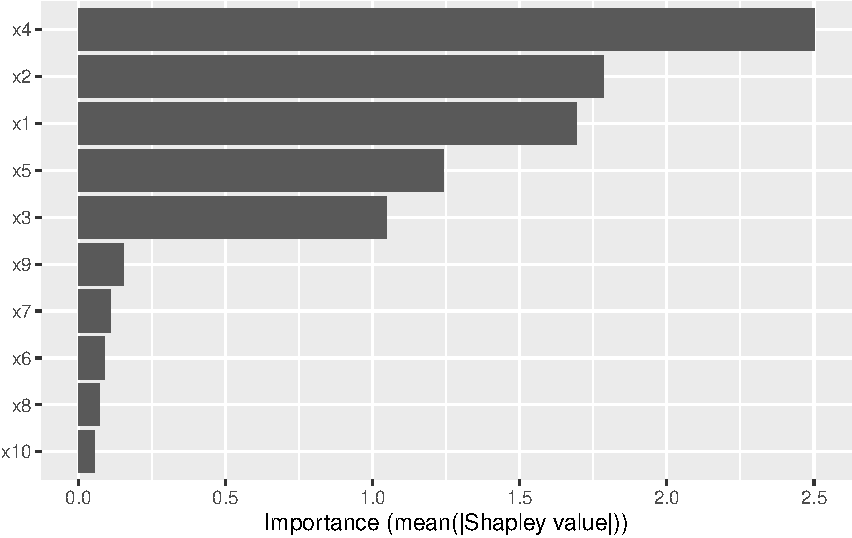
\includegraphics[width=0.7\linewidth]{greenwell-boehmke_files/figure-latex/vi-shap-1}

}

\caption[Shapley-based VI scores from an XGBoost model fit to the simulated Friedman data]{Shapley-based VI scores from an XGBoost model fit to the simulated Friedman data.}\label{fig:vi-shap}
\end{figure}
\end{Schunk}

\section{Drawbacks of existing methods}

As discussed in \citet{hooker-2019-stop}, \dfn{permute-and-predict}
methods---like PDPs, ICE curves, and permutation importance---can
produce results that are highly misleading.\footnote{It's been argued
  that approximate Shapley values share the same drawback, however,
  \citet{janzing-2019-feature} makes a compelling case against those
  arguments.} For example, the standard approach to computing
permutation-based VI scores involves independently permuting individual
features. This implicitly makes the assumption that the observed
features are statistically independent. In practice, however, features
are often not independent which can lead to nonsensical VI scores. One
way to mitigate this issue is to use the conditional approach described
in \citet{strobl-2019-conditional}; \citet{hooker-2019-stop} provides
additional alternatives, such as \dfn{permute-and-relearn importance}.
Unfortunately, to the best of our knowledge, this approach is not yet
available for general purpose. A similar modification can be applied to
PDPs \citep{parr-2019-technical}\footnote{A basic R implementation is
  available at \url{https://github.com/bgreenwell/rstratx}.} which seems
reasonable to use in the FIRM approach when strong dependencies among
the features are present (though, we have not given this much thought or
consideration).

We already mentioned that PDPs can be misleading in the presence of
strong interaction effects. This drawback, of course, equally applies to
the FIRM approach using PDPs for computing VI scores. As discussed
earlier, this can be mitigated by using ICE curves instead. Another
alternative would be to use \dfn{accumulated local effect} (ALE) plots
\citep{apley-2016-visualizing} (though we haven't really tested this
idea). Compared to PDPs, ALE plots have the advantage of being faster to
compute and less affected by strong dependencies among the features. The
downside, however, is that ALE plots are more complicated to implement
(hence, they are not currently available when using
\code{method = "firm"}). ALE plots are available in the
\CRANpkg{ALEPlot} \citep{R-ALEPlot} and \pkg{iml} packages.

\citet{hooker-2007-generalized} also argues that feature importance
(which concern only \dfn{main effects}) can be misleading in high
dimensional settings, especially when there are strong dependencies and
interaction effects among the features, and suggests an approach based
on a \dfn{generalized functional ANOVA decomposition}---though, to our
knowledge, this approach is not widely implemented in open source.

\section{Use sparklines to characterize feature effects}

Starting with \pkg{vip} 0.1.3, we have included a new function
\code{add\_sparklines()} for constructing HTML-based VI tables; however,
this feature requires the \CRANpkg{DT} package \citep{R-DT}. The primary
difference between \code{vi()} and \code{add\_sparklines()} is that the
latter includes an \code{Effect} column that displays a sparkline
representation of the partial dependence function for each feature. This
is a concise way to display both feature importance and feature effect
information in a single (interactive) table. See
\code{?vip::add\_sparklines} for details. We illustrate the basic use of
\code{add\_sparklines()} in the code chunk below where we fit a
\pkg{ranger}-based random forest using the \CRANpkg{mlr3} package
\citep{R-mlr3}.\footnote{\textbf{Note:} Here we use the \texttt{...}
  argument to pass the original training to \texttt{pdp::partial()};
  this is to avoid conflicts caused by \pkg{mlr3}'s \CRANpkg{data.table}
  backend \citep{R-data.table}.}

\begin{Schunk}
\begin{Sinput}
# Load required packages
library(mlr3)
library(mlr3learners)

# Fit a ranger-based random forest using the mlr3 package
set.seed(101)
task <- TaskRegr$new("friedman", backend = trn, target = "y")
lrnr <- lrn("regr.ranger", importance = "impurity")
lrnr$train(task)

# First, compute a tibble of VI scores using any method
var_imp <- vi(lrnr)

# Next, convert to an HTML-based data table with sparklines
add_sparklines(var_imp, fit = lrnr$model, train = trn)  # Figure 18
\end{Sinput}
\begin{figure}[!htb]

{\centering 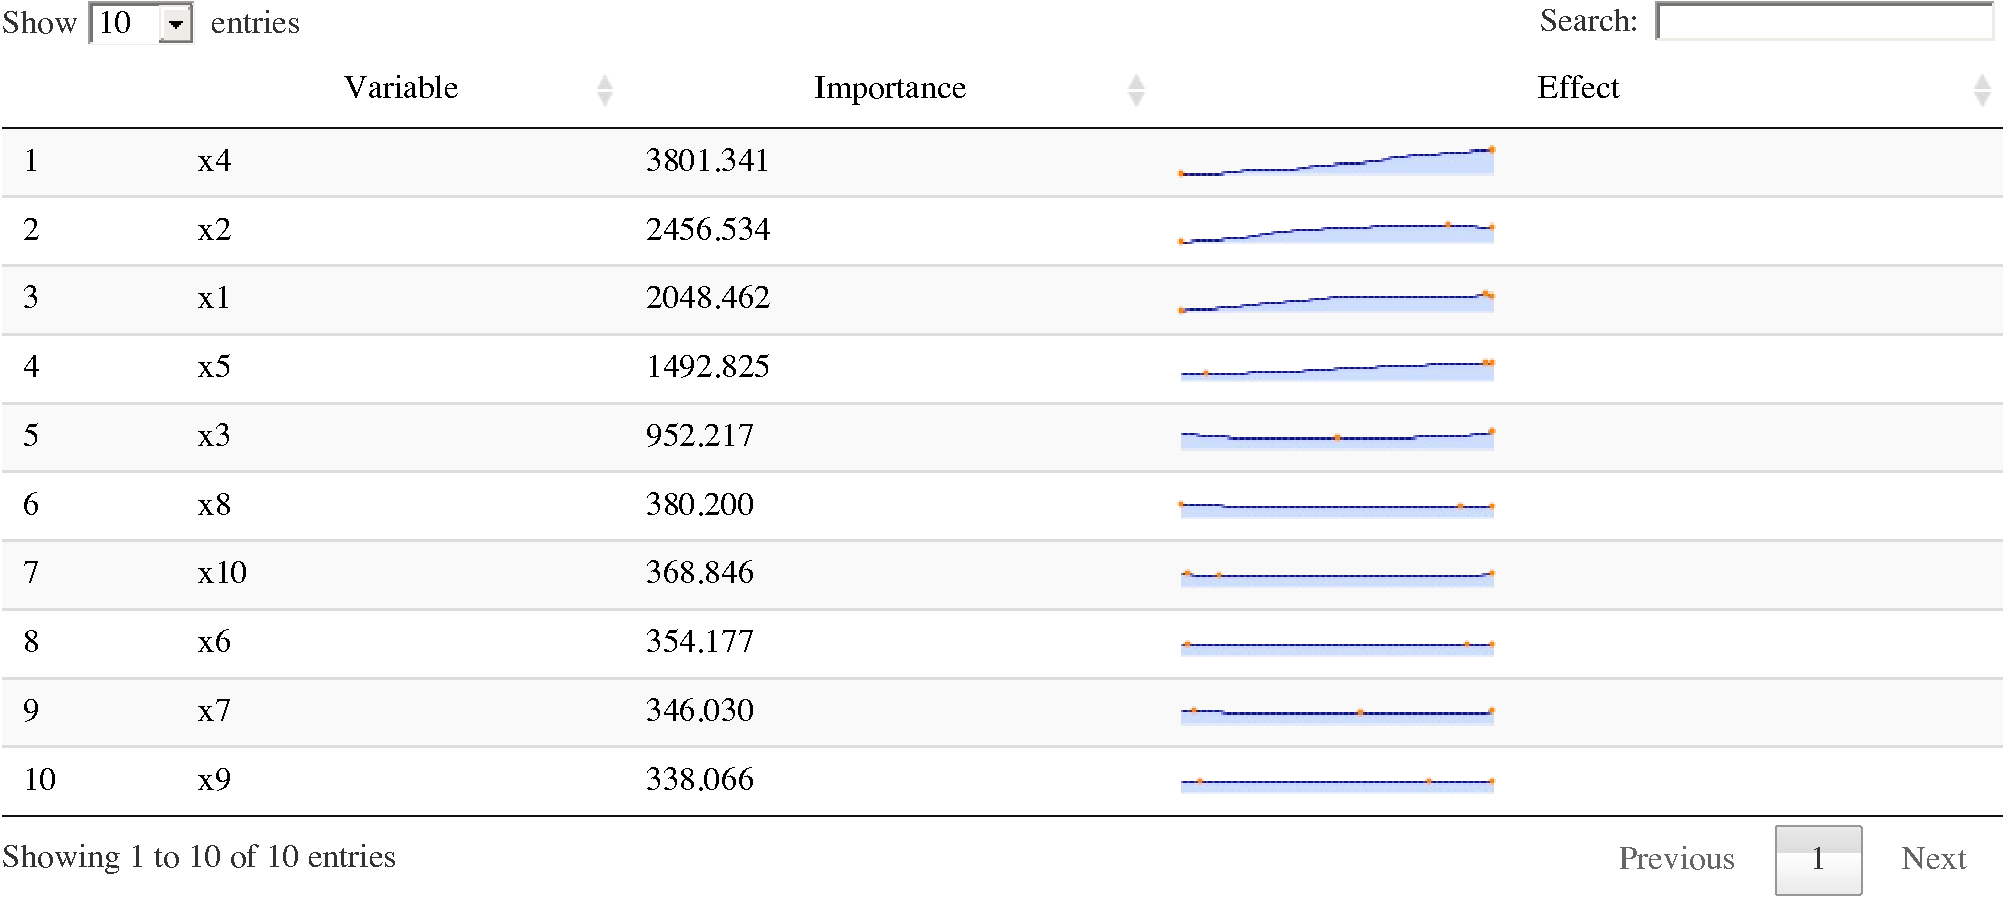
\includegraphics[width=1\linewidth]{greenwell-boehmke_files/figure-latex/sparklines-1}

}

\caption[Variable importance scores along with a sparkline representation of feature effects]{Variable importance scores along with a sparkline representation of feature effects.}\label{fig:sparklines}
\end{figure}
\end{Schunk}

\section{Ames housing example}

For illustration, we'll use the Ames housing data \citep{ames-cock-2011}
which are available in the \CRANpkg{AmesHousing} package
\citep{R-AmesHousing}. These data describe the sale of individual
residential properties in Ames, Iowa from 2006--2010. The data set
contains 2930 observations, 80 features (23 nominal, 23 ordinal, 14
discrete, and 20 continuous), and a continuous target giving the sale
price of the home. The version we'll load is a cleaned up version of the
original data set and treats all categorical variables as nominal (see
\code{?AmesHousing::make\_ames} for details).

Using the R package \CRANpkg{SuperLearner} \citep{R-SuperLearner}, we
trained five models using 5-fold cross-validation: a GBM using the
\pkg{xgboost} package, an RF using the \pkg{ranger} package, a MARS
model using the \pkg{earth} package, a GLMNET model using the
\CRANpkg{glmnet} package \citep{R-glmnet}, and a support vector
regression model using the \CRANpkg{kernlab} package \citep{R-kernlab}.
The magnitude of the coefficients from the meta learner indicate which
models contribute the most (if at all) to new predictions.

\begin{Schunk}
\begin{Sinput}
# Load the Ames housing data
ames <- AmesHousing::make_ames()
X <- subset(ames, select = -Sale_Price)
y <- ames$Sale_Price

# Load required packages
library(SuperLearner)

# List of base learners
learners <- c("SL.xgboost", "SL.ranger", "SL.earth", "SL.glmnet", "SL.ksvm")

# Stack models
set.seed(840)  # for reproducibility
ctrl <- SuperLearner.CV.control(V = 5L, shuffle = TRUE)
sl <- SuperLearner(Y = y, X = X, SL.library = learners, verbose = TRUE,
                   cvControl = ctrl)
sl
\end{Sinput}
\begin{Soutput}
#>
#> Call:
#> SuperLearner(Y = y, X = X, SL.library = learners, verbose = TRUE, cvControl = ctrl)
#>
#>
#>
#>                      Risk       Coef
#> SL.xgboost_All  569646381 0.43455425
#> SL.ranger_All   666208088 0.06970309
#> SL.earth_All    553872844 0.49574265
#> SL.glmnet_All   908881559 0.00000000
#> SL.ksvm_All    6784289108 0.00000000
\end{Soutput}
\end{Schunk}

In the code chunks below we request permutation-based VI scores and a
sparkline representation of the PDPs for the top ten features. For this
we need to define a couple of wrapper functions: one for computing
predictions (for the permutation VI scores), and one for computing
averaged predictions (for the PDPs).

\begin{Schunk}
\begin{Sinput}
# Prediction wrapper functions
imp_fun <- function(object, newdata) {  # for permutation-based VI scores
  predict(object, newdata = newdata)$pred
}
par_fun <- function(object, newdata) {  # for PDPs
  mean(predict(object, newdata = newdata)$pred)
}
\end{Sinput}
\end{Schunk}

To speed up the process, we perform the computations in parallel by
setting \code{parallel = TRUE} in the calls to \code{vi()} and
\code{add\_sparklines()}. Note that we first need to set up a parallel
backend for this to work. Both \pkg{vip} and \pkg{pdp} use
\CRANpkg{plyr} \citep{R-plyr}---which relies on \pkg{foreach}---so any
parallel backend supported by the \pkg{foreach} package should work.
Below we use a \dfn{socket} approach with the \CRANpkg{doParallel}
backend \citep{R-doParallel} using a cluster of size five.

\begin{Schunk}
\begin{Sinput}
# Setup parallel backend
library(doParallel) # load the parallel backend
cl <- makeCluster(5) # use 5 workers
registerDoParallel(cl) # register the parallel backend

# Permutation-based feature importance
set.seed(278)  # for reproducibility
var_imp <- vi(sl, method = "permute", train = X, target = y, metric = "rmse",
              pred_wrapper = imp_fun, nsim = 5, parallel = TRUE)

# Add sparkline representation of feature effects (# Figure 19)
add_sparklines(var_imp[1L:10L, ], fit = sl, pred.fun = par_fun, train = X,
               digits = 2, verbose = TRUE, trim.outliers = TRUE,
               grid.resolution = 20, parallel = TRUE)
\end{Sinput}
\begin{figure}[!htb]

{\centering 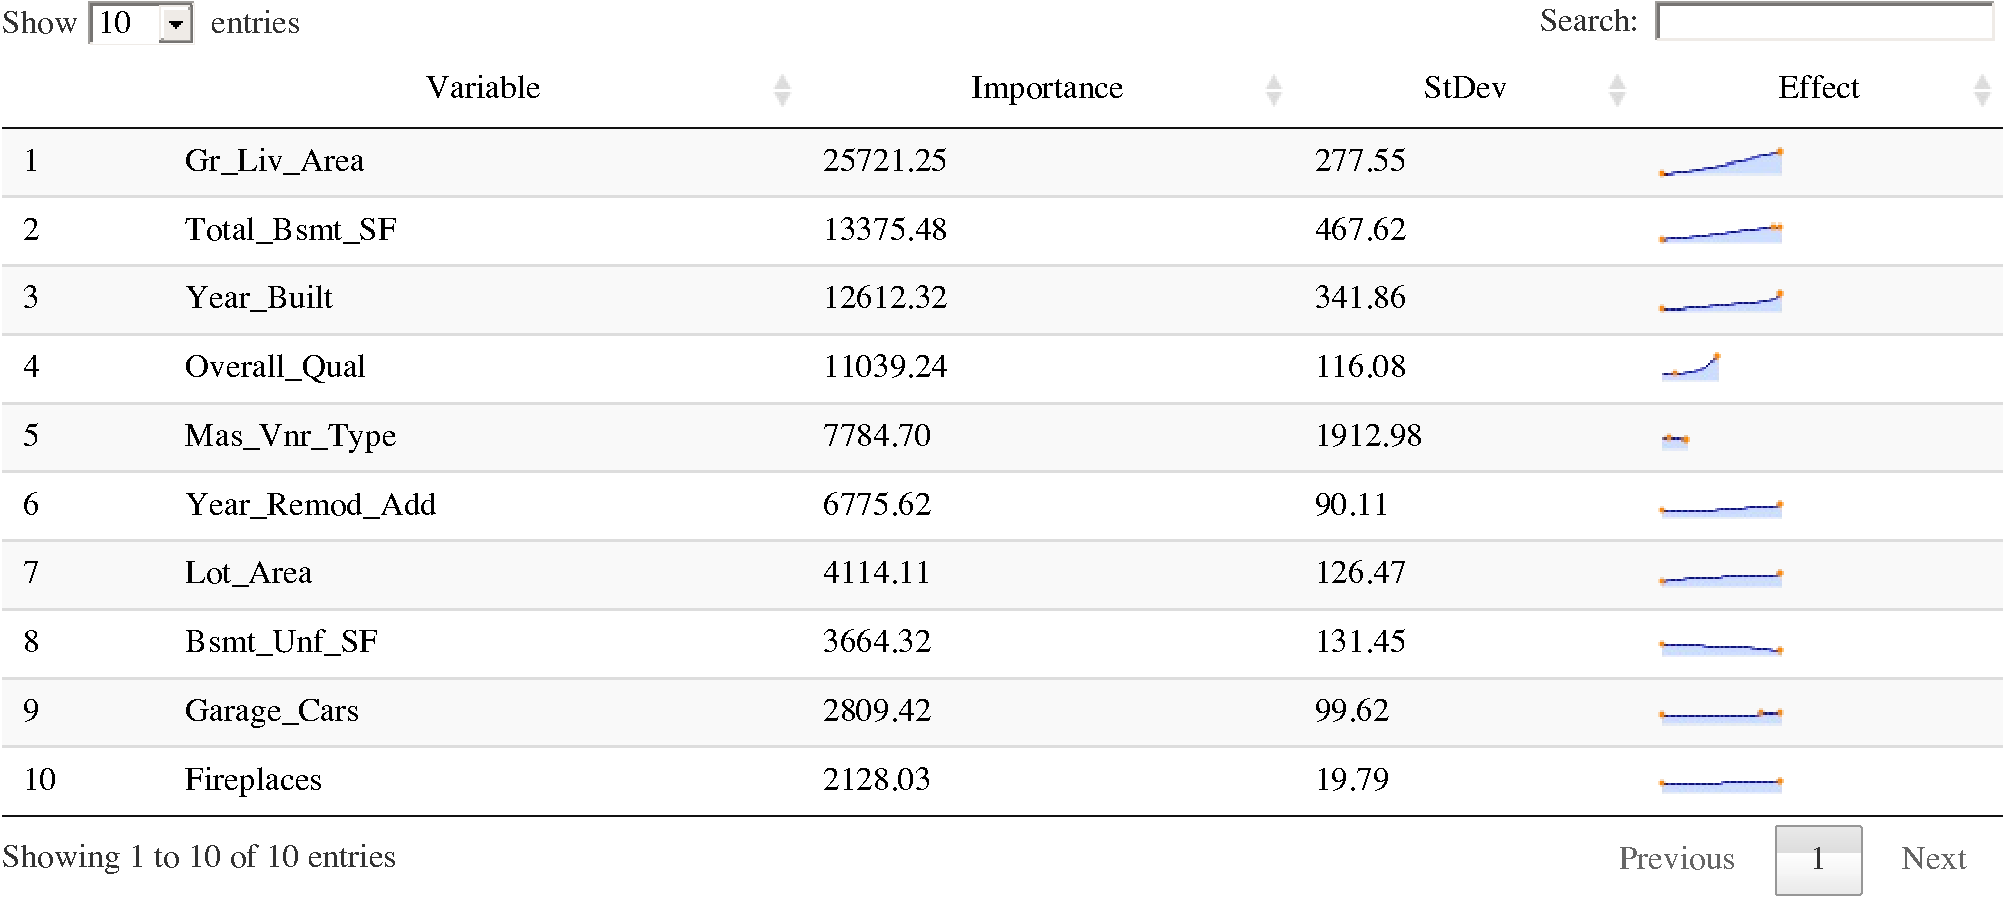
\includegraphics[width=1\linewidth]{greenwell-boehmke_files/figure-latex/ames-sparklines-1}

}

\caption[VIP with sparkline representation of feature effects for the top ten features from a Super Learner fit to the Ames housing data]{VIP with sparkline representation of feature effects for the top ten features from a Super Learner fit to the Ames housing data.}\label{fig:ames-sparklines}
\end{figure}
\begin{Sinput}
# Shut down cluster
stopCluster(cl)
\end{Sinput}
\end{Schunk}

\section{Summary}

VIPs help to visualize the strength of the relationship between each
feature and the predicted response, while accounting for all the other
features in the model. We've discussed two types of VI: model-specific
and model-agnostic, as well as some of their strengths and weaknesses.
In this paper, we showed how to construct VIPs for various types of
``black box'' models in R using the \pkg{vip} package. We also briefly
discussed related approaches available in a number of other R packages.
Suggestions to avoid high execution times were discussed and
demonstrated via examples. This paper is based on \pkg{vip} version
0.2.1. In terms of future development, \pkg{vip} can be expanded in a
number of ways. For example, we plan to incorporate the option to
compute group-based and conditional permutation scores. Although not
discussed in this paper, \pkg{vip} also includes a promising statistic
(similar to the variance-based VI scores previously discussed) for
measuring the relative strength of interaction between features.
Although VIPs can help understand which features are driving the model's
predictions, ML practitioners should be cognizant of the fact that none
of the methods discussed in this paper are uniformly best across all
situations; they require an accurate model that has been properly tuned,
and should be checked for consistency with human domain knowledge.

\section{Acknowledgments}

The authors would like to thank the anonymous reviewers and the Editor
for their helpful comments and suggestions. We would also like to thank
the members of the 84.51\(^{\circ}\) Interpretable Machine Learning
Special Interest Group for their thoughtful discussions on the topics
discussed herein.

\bibliography{greenwell-boehmke}


\address{%
Brandon M. Greenwell\\
University of Cincinnati\\
2925 Campus Green Dr\\ Cincinnati, OH 45221\\ United States of America\\ ORCiD---\href{https://orcid.org/0000-0002-8120-0084}{0000-0002-8120-0084}\\
}
\href{mailto:greenwell.brandon@gmail.com}{\nolinkurl{greenwell.brandon@gmail.com}}

\address{%
Bradley C. Boehmke\\
University of Cincinnati\\
2925 Campus Green Dr\\ Cincinnati, OH 45221\\ United States of America\\ ORCiD---\href{https://orcid.org/0000-0002-3611-8516}{0000-0002-3611-8516}\\
}
\href{mailto:bradleyboehmke@gmail.com}{\nolinkurl{bradleyboehmke@gmail.com}}

